% $Header$

\documentclass{beamer}

\mode<presentation>
{
  %\usetheme{CambridgeUS}
  %\usecolortheme{seahorse}
  \usetheme{Warsaw}
  \usecolortheme{seahorse}

  \setbeamercovered{transparent}
  % or whatever (possibly just delete it)
}

\usepackage{verbatim}
\usepackage[english]{babel}
\usepackage{fancybox}
% or whatever

\usepackage[latin1]{inputenc}
% or whatever

\usepackage{times}
\usepackage[T1]{fontenc}
% Or whatever. Note that the encoding and the font should match. If T1
% does not look nice, try deleting the line with the fontenc.

\setbeamerfont{title}{shape=\itshape,family=\rmfamily}
\title[Black hole entropy function with CS-terms]
{The black hole entropy function in the presence of 
a gauge Chern-Simons term in five dimensions}


\author[H.~Jennen]{Hendrik Jennen\\
[10pt]{\footnotesize Supervisor: Dr.\ Jan Perz}}
% - Give the names in the same order as the appear in the paper.
% - Use the \inst{?} command only if the authors have different
%   affiliation.



\date{June 24, 2010}
% - Either use conference name or its abbreviation.
% - Not really informative to the audience, more for people (including
%   yourself) who are reading the slides online

\subject{Master's thesis}
% This is only inserted into the PDF information catalog. Can be left
% out. 


% If you have a file called "university-logo-filename.xxx", where xxx
% is a graphic format that can be processed by latex or pdflatex,
% resp., then you can add a logo as follows:

\pgfdeclareimage[height=0.5cm]{university-logo}{sedes.png}
\logo{\pgfuseimage{university-logo}}



% Delete this, if you do not want the table of contents to pop up at
% the beginning of each subsection:
\begin{comment}
\AtBeginSubsection[]
{
  \begin{frame}<beamer>{Outline}
    \tableofcontents[currentsection,currentsubsection]
  \end{frame}
}
\end{comment}


% If you wish to uncover everything in a step-wise fashion, uncomment
% the following command: 

%\beamerdefaultoverlayspecification{<+->}


\begin{document}

\begin{frame}
  \titlepage
\end{frame}

\begin{frame}{Outline}
  \tableofcontents
  % You might wish to add the option [pausesections]
\end{frame}


% Structuring a talk is a difficult task and the following structure
% may not be suitable. Here are some rules that apply for this
% solution: 

% - Exactly two or three sections (other than the summary).
% - At *most* three subsections per section.
% - Talk about 30s to 2min per frame. So there should be between about
%   15 and 30 frames, all told.

% - A conference audience is likely to know very little of what you
%   are going to talk about. So *simplify*!
% - In a 20min talk, getting the main ideas across is hard
%   enough. Leave out details, even if it means being less precise than
%   you think necessary.
% - If you omit details that are vital to the proof/implementation,
%   just say so once. Everybody will be happy with that.

%%%%%%%%
\section{Gravity and electrodynamics}

%%%%
\subsection{Einstein-Maxwell theory}

\begin{frame}{Equations of motion: Einstein's equations}

  \begin{block}{Action}
  \begin{displaymath}
  \mathcal{S} = \int  R \star 1 
  \uncover<2->{\alert<2>{- F\wedge \star F}}
  \end{displaymath}
  \end{block}
  
  \begin{itemize}
  \item Einstein's equations (metric eqs.~of motion)
    \begin{align*}
    R_{\mu\nu} - \frac{1}{2} R\, g_{\mu\nu} &= \only<1>{0}
    \only<2->{\alert<2>{ T_{\mu\nu}}}\\
    \visible<3->{
    \mathrm{geometry} &\leftrightarrow \mathrm{energy}}
    \end{align*}
    
  \visible<4->{
  \item Finding a generic solution is highly non-trivial
    \begin{itemize}
    \item Anticipate solutions with symmetry: Ans\"atze
    \end{itemize}}
    
  \end{itemize}
\end{frame}

%%%%
\subsection{Black holes and thermodynamics}

\begin{frame}{Black hole solutions}

  \begin{itemize}
  \item Charged $(q)$ non-rotating mass $(M)$ at ``origin''
    \begin{itemize}
    \item Static spherically symmetric Ansatz
    \end{itemize}
    
  \visible<2->{
    \begin{block}{Space-time metric (Reissner-Nordstr\"om)}
    \begin{displaymath}
      ds^{2} =  - \Delta(r) dt^{2} +  \Delta^{-1}(r)dr^{2} + r^{2} d\Omega_{2}
      \end{displaymath}
    \end{block}
  
  \uncover<3->{  
  \item $\Delta(r)$ has two coordinate singularities $r_{\pm} = M \pm \sqrt{M^{2} - q^{2}}$
    \begin{itemize}
    \item Horizons---black hole
    %\item Cosmic censorship hypothesis
    \end{itemize}
  }
  
  \uncover<4->{  
  \item If $M = q$: black hole is \alert{extremal}
    \begin{itemize}
    \item Maximal charge for given mass
    \end{itemize}
    }
  }
  \end{itemize}

  
\end{frame}

\begin{frame}{Black hole thermodynamics}

  \begin{itemize}
  \item Classically black holes cannot radiate
  \pause
    \begin{itemize}
    \item Zero temperature
    \end{itemize}
   
   \pause 
   \item Laws of black hole mechanics
     \begin{itemize}
     \item Reminiscent of laws of thermodynamics
     \item E.g.\ black hole horizon area never decreases
     \pause
     \item Macroscopic entropy $\sim$ area? [Bekenstein]
     \end{itemize}
  
  \pause  
  \item Quantum field theory on classical curved background
    \begin{itemize}
    \item Thermodynamical spectrum of black body [Hawking]
    \end{itemize}
    
    \begin{displaymath}
    S = \frac{A}{4\hbar}  
    \end{displaymath}
  \end{itemize}
  
\end{frame}

%%%%
\subsection{Generalized Einstein-Maxwell theory}

\begin{frame}{Generalized Einstein-Maxwell theory}

  \begin{block}{action}
    \begin{displaymath}
    \mathcal{S} = \int  R \star 1 - g_{rs}(\varphi) d\varphi^{r} \wedge \star d\varphi^{s} -
    	\alert<2>{h_{ij}(\varphi)} F^{i} \wedge \star F^{j} 
    \end{displaymath}
  \end{block}

  \begin{itemize}
  \item Gravitation coupled to a set of scalar and vector fields
  \pause
  \item Coupling matrices $g_{rs}$ and $h_{ij}$ depend on scalars
  \pause
  \item No potential terms
  \item Static spherically symmetric extremal black hole solutions
  \item Einstein-Maxwell: special case
  \vspace{5mm}
  \item Structure suggested by supergravity (bosonic sector)
  
  \end{itemize}

\end{frame}


%%%%%%%%
\section{The entropy function formalism}

%%%%
\subsection{The attractor mechanism}

\begin{frame}{The attractor mechanism}

\only<1-3,5->{
  \begin{itemize}
  \item Non-trivial dynamics only in \alert<1>{radial} direction
    \begin{itemize}
    \item<1-> Static spherically symmetric extremal black holes
    \end{itemize}
  
  \item<2-> Integrate out the fields along other directions
    \begin{displaymath}
    \mathcal{S}_{\mathrm{eff}} = \int dr \, g_{ij} \dot{\varphi}^{i} \dot{\varphi}^{j}(r)
    	+ \alert<3>{V_{\mathrm{BH}}(\phi^{i},q)} + [\ldots]
    \end{displaymath}
    
  \item<3-> Effective potential for the scalars
    \begin{itemize}
    \item Scalars at horizon do not depend on asymptotic values: $\varphi^{i}_{\mathrm{H}}(q)$
    \item Attractor mechanism
    \end{itemize}
}  
    
\only<4>{
  \begin{figure}
  \centering
  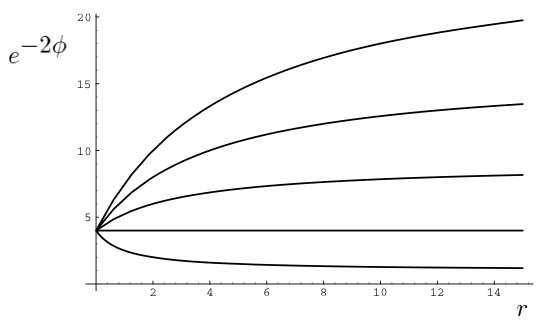
\includegraphics[width=9cm]{attractorflow.png}
  \caption{Adapted from arXiv:0805.2498v2 [hep-th]}
  \end{figure}
}  

\only<1-3,5->{    
  \item<4-> Macroscopic entropy depends on charges only
    \begin{displaymath}
    S \sim \mathrm{Area}(\varphi^{i}_{\mathrm{H}}(q),q)
    \end{displaymath}
    \visible<5->{
    $\rightarrow$ Importance of attractor mechanism}
  \end{itemize}
}

\end{frame}



%%%%
\subsection{The entropy function}

\begin{frame}{The entropy function}

  \begin{itemize}
  
  \item Goal: function with two practical properties
    \begin{itemize}
    \item On-shell fields at horizon---variational principle
    \item Entropy at extremum
    \end{itemize}
  \visible<2->{
  \uncover<2->{
  \item No explicit dependence on gauge potentials}
  \uncover<3->{
  \item Assume symmetry}
  \uncover<4->{
  \item How? Legendre transform w.r.t.\ e-fields}
  
  \begin{block}{\uncover<4->{Entropy function [Sen]}}
    \begin{displaymath}
    \uncover<4->{\mathcal{E} \equiv q_{i}e^{i} -}
    \uncover<3->{\int_{\mathrm{H}} d\theta\, d\phi\,}
    \mathcal{L}(g,\varphi^{s},F^{i})
    \end{displaymath}
  \end{block}}
  
  \visible<5->{
  \item Attractor mechanism}
  \end{itemize}

\end{frame}


%%%%%%%%
\section{Five dimensions: Chern-Simons terms}

%%%%
\subsection{Maxwell charge vs.\ Page charge}

\begin{frame}{Chern-Simons term and Page charge}

  \begin{block}{Action - 5D}
  \begin{displaymath}
  \mathcal{S} = \int  F\wedge \star F + \alert<1>{A \wedge F \wedge F} + [\ldots]
  \end{displaymath}
  \end{block}

  \begin{columns}[t]
  \column{.3\textwidth}
  \uncover<2->{
    \begin{displaymath}
    d\star F = -  \frac{3}{2} F \wedge F
    \end{displaymath}}\\
    \uncover<4->{
    \begin{block}{\center Maxwell charge}
      \begin{itemize}
      \item Conserved
      \item Not localized
      \end{itemize}
    \end{block}}
    
     
    \column{0.20\textwidth}
    \uncover<2->{
      \begin{displaymath}\Longleftrightarrow
      \end{displaymath}}\\
    \uncover<3->{     
      \begin{displaymath}
      Q \equiv \int d(\ldots)
      \end{displaymath}}
   
  \column{.3\textwidth}
  \uncover<2->{
    \begin{displaymath}
    d(\star F + \frac{3}{2} A \wedge F) = 0
    \end{displaymath}}\\
    \uncover<5->{
    \begin{block}{\center Page charge}
      \begin{itemize}
      \item Conserved
      \item \alert{Localized}
      \end{itemize}
    \end{block}}
    
  \end{columns}
  

\end{frame}

%%%%
\subsection{Two proposals}

\begin{frame}{Dimensional reduction {\footnotesize [Cardoso, Oberreuter, Perz; Goldstein, Jena] }}

  \begin{itemize}
  \item Establish connection between 5D and 4D black holes
  \end{itemize}
  \begin{figure}
  \centering
  \visible<2->{
  \includegraphics[width=8cm]{taub-NUT.png}}
  \end{figure}
    %%%%%%
   % \begin{comment}
    %\item 5D black hole with asymptotic Taub-NUT geometry
     % \begin{itemize}
      %\item $\mathbb{R}^{3} \times S^{1}$: 1 compact direction---a circle (space part)
      %\end{itemize}
    
   % \pause  
    %\item Reduction along circle gives effective 4D description
      %\begin{itemize}
      %\item Entropy function well-defined for this 4D black hole
      %\end{itemize}
    %\end{comment}
    %%%%%%
  \uncover<3->{
  \begin{block}{Entropy function with CS-terms (1)}\center
    entropy function 5D black hole\\ $\equiv$\\
    entropy function associated 4D black hole
  \end{block}}
  
\end{frame}

\begin{frame}{Direct 5D procedure {\footnotesize [Arsiwalla]}}

  \begin{itemize}
    \item Entropy function defined analogously as in 4D
    \item<2-> Integrate Lagrangian along horizon of black hole
    \item<3-> Charges conjugate to e-fields
    \item<4-> Entropy function as Legendre transform
   \end{itemize}
   
  \begin{columns}[c]
   
  \column{0.35\textwidth}
    \begin{block}{\center 4D}
      \begin{itemize}
      \item<2-> $\mathcal{F}_{4}$
      \item<3-> $q = \partial \mathcal{F}_{4} / \partial e$
      \item<4-> $\mathcal{E}_{4} \equiv qe - \mathcal{F}_{4}$
      \end{itemize}
    
    \end{block}
    
  \column{0.03\textwidth}
    $\rightarrow$
    
  
  \column{0.35\textwidth}
    \begin{block}{\center 5D}
      \begin{itemize}
      \item<2-> $\mathcal{F}_{5}$
      \item<3-> \alert<5>{$Q \alert<3>{\equiv} \partial \mathcal{F}_{5} / \partial e$
      		\visible<5>{ (?)}}
      \item<4-> $\mathcal{E}_{5} \equiv Qe - \mathcal{F}_{5}$
      \end{itemize}
    
    \end{block}
  
  \end{columns}
  
\end{frame}

\begin{frame}{Direct 5D procedure - discussion}

  \begin{itemize}
  \item $Q$ the Page charge?
  		\visible<2->{\alert<2>{No.}}
  \uncover<2->{
    \begin{itemize}
      \item Mismatch in relative factors due to CS-terms
      \item Explicit appearance of gauge potentials
    \end{itemize}
  }
  
  \uncover<3->{
  \begin{block}{}
      When action depends explicitly on gauge potentials the conjugate charges are not
      conserved quantities.
  \end{block}
  }
  
  \item<4-> EF as Legendre transform w.r.t.\ e-fields not possible
  
  \visible<5->{
  \item However: Page charge seems right quantity for EF
    \begin{itemize}
    \item Consistency with attractor mechanism
    \end{itemize}
  }
  
  \end{itemize}    


\end{frame}

\section*{Conclusion}

\begin{frame}{Conclusion}

  % Keep the summary *very short*.
  \begin{itemize}
  \item
    We compared two proposals to extend the entropy function to BH solutions in the 
    presence of CS-terms (5D).
  \item
    Page charge is the natural quantity to use in a 5D entropy function as it is measurable 
    at the horizon.
  \item
    Entropy function defined as a Legendre transform w.r.t.\ the electric fields seems
    not possible due to explicit gauge potentials in the action.

  \end{itemize}
  
  % The following outlook is optional.
  \vskip0pt plus.5fill
  \begin{itemize}
  \item
    Outlook
    \begin{itemize}
    \item
      Dimensional reduction of black holes with other asymptotic geometries
    \item
      Entropy function not as Legendre transform in five dimensions
    \end{itemize}
  \end{itemize}
\end{frame}


\begin{comment}
% All of the following is optional and typically not needed. 
\appendix
\section<presentation>*{\appendixname}
\subsection<presentation>*{For Further Reading}

\begin{frame}[allowframebreaks]
  \frametitle<presentation>{For Further Reading}
    
  \begin{thebibliography}{10}
    
  \beamertemplatebookbibitems
  % Start with overview books.

  \bibitem{Author1990}
    A.~Author.
    \newblock {\em Handbook of Everything}.
    \newblock Some Press, 1990.
 
    
  \beamertemplatearticlebibitems
  % Followed by interesting articles. Keep the list short. 

  \bibitem{Someone2000}
    S.~Someone.
    \newblock On this and that.
    \newblock {\em Journal of This and That}, 2(1):50--100,
    2000.
  \end{thebibliography}
\end{frame}
\end{comment}

\begin{frame}

\end{frame}


\end{document}


